\documentclass[a4paper,12pt]{article}
\usepackage[utf8]{inputenc}
\usepackage[T1]{fontenc}
\usepackage[italian]{babel}
\usepackage{graphicx}
\usepackage{caption}
\usepackage{geometry}
\usepackage{hyperref}
\usepackage{float}

\geometry{margin=2.5cm}

\graphicspath{{./immagini/}}

\title{\textbf{Setup delle Macchine Virtuali}\\
	\large Guida per l'esame di Sicurezza Informatica}
\author{Elia Cruciat}
\date{17/06/2026}

\begin{document}
	
	\maketitle
	\tableofcontents
	\newpage
	
	% ─────────────────────────────────────────────
	\section{Creazione della macchina virtuale}
	
	Aprire VirtualBox e creare una nuova macchina virtuale seguendo le tre fasi illustrate di seguito.
	In laboratorio, il disco virtuale da selezionare nella terza fase si trova sempre nella stessa cartella predisposta dai tecnici.
	
	\begin{figure}[H]
		\centering
		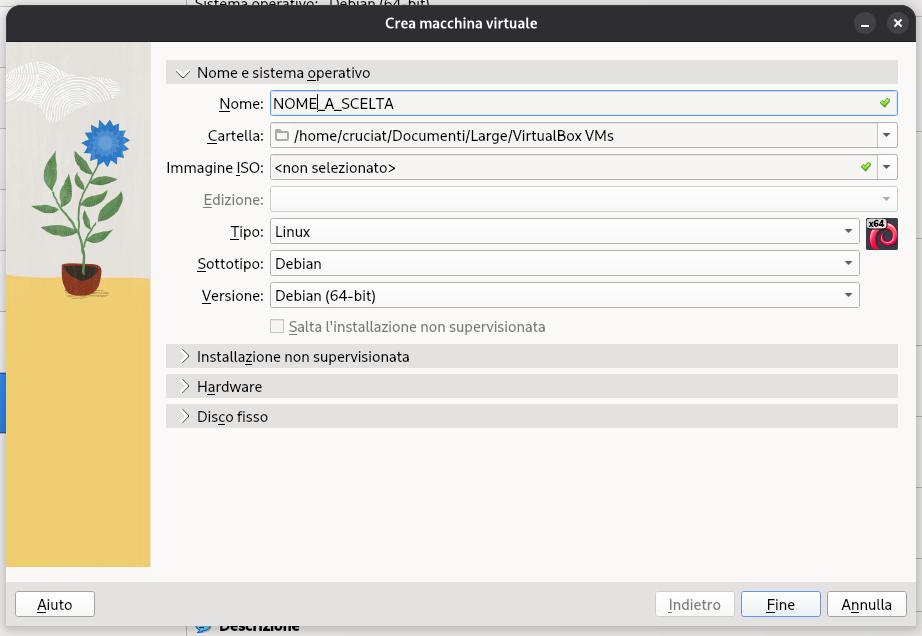
\includegraphics[width=0.85\textwidth]{creation1.png}
		\caption{Fase 1 — Impostare il nome della VM, il tipo (\texttt{Linux}), il sottotipo (\texttt{Debian}) e la versione (\texttt{Debian (64-bit)}).}
		\label{fig:creation1}
	\end{figure}
	
	\begin{figure}[H]
		\centering
		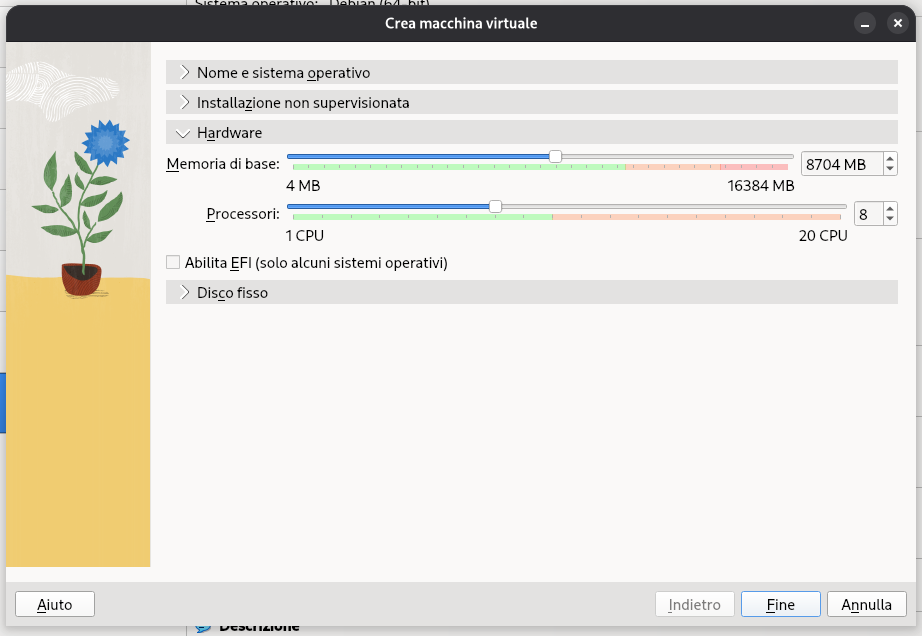
\includegraphics[width=0.85\textwidth]{creation2.png}
		\caption{Fase 2 — Assegnare le risorse hardware: quantità di memoria RAM e numero di processori virtuali.}
		\label{fig:creation2}
	\end{figure}
	
	\begin{figure}[H]
		\centering
		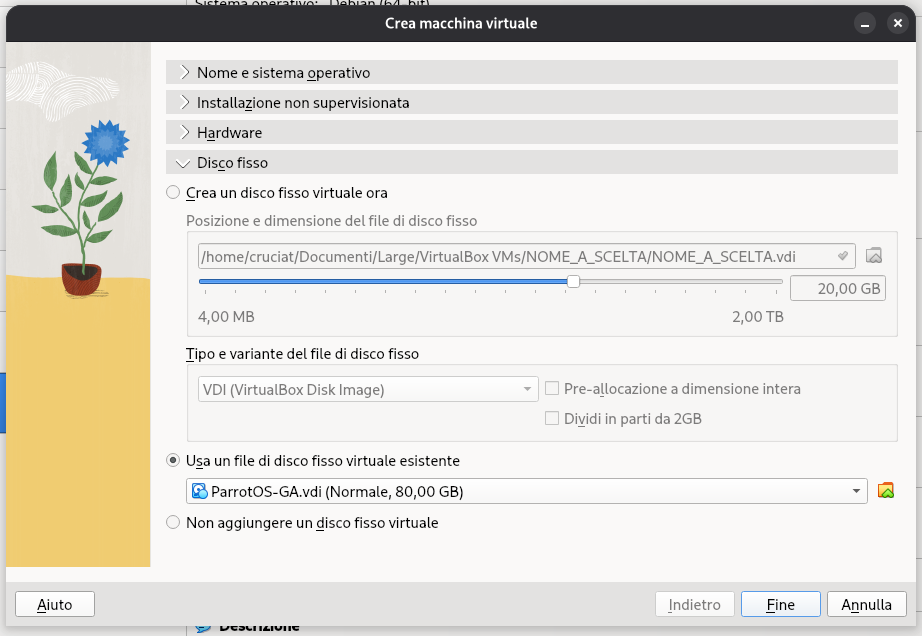
\includegraphics[width=0.85\textwidth]{creation3.png}
		\caption{Fase 3 — Selezionare \textit{Usa un disco fisso virtuale esistente} e scegliere il file \texttt{.vdi} dalla cartella indicata dal laboratorio.}
		\label{fig:creation3}
	\end{figure}
	
	% ─────────────────────────────────────────────
	\section{Configurazione delle impostazioni}
	
	Prima di avviare, vanno modificate alcune cose nel pannello \textbf{Impostazioni} della VM.
	
	\subsection{Generale — Avanzate}
	
	\begin{figure}[H]
		\centering
		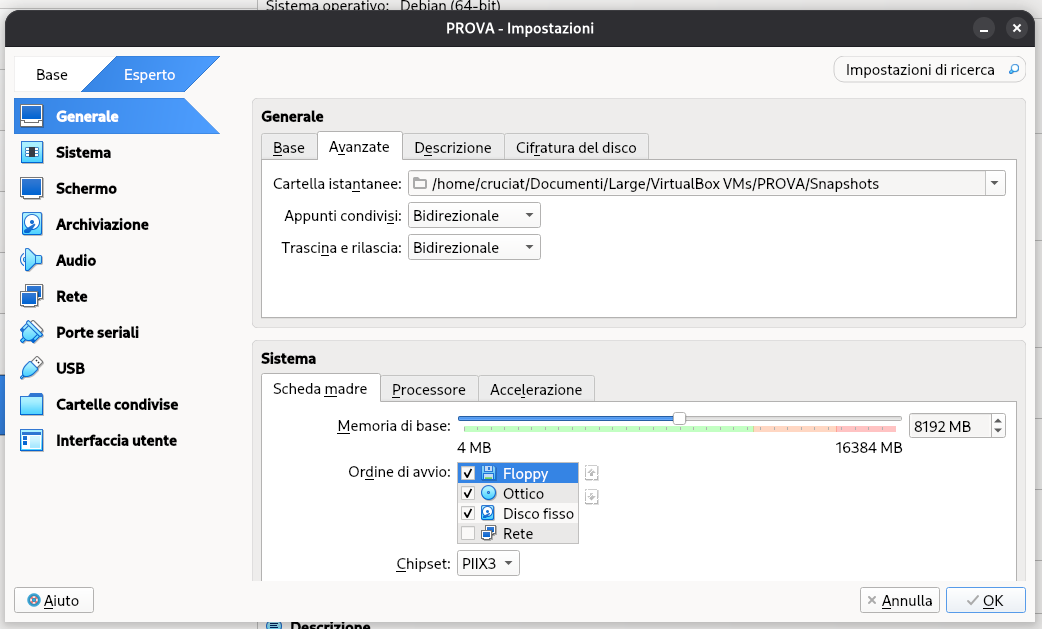
\includegraphics[width=0.85\textwidth]{clipboard.png}
		\caption{In \textit{Impostazioni > Generale > Avanzate}, impostare sia \textbf{Appunti condivisi} che \textbf{Trascina e rilascia} su \textbf{Bidirezionale}. È utile annotare anche il percorso della cartella \textit{Istantanee}, poiché contiene gli screenshot catturati dall'interno della VM.}
		\label{fig:clipboard}
	\end{figure}
	
	\subsection{Rete — Scheda 2}
	
	La scheda 1 è già configurata correttamente. Basta attivare e configurare la scheda 2.
	
	\begin{figure}[H]
		\centering
		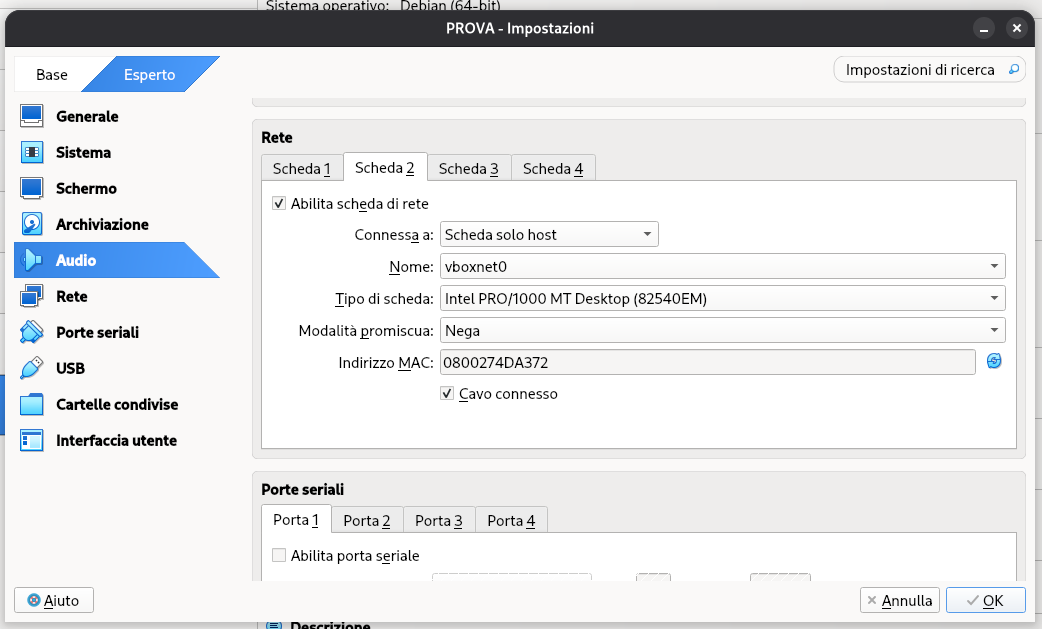
\includegraphics[width=0.85\textwidth]{host_only_adapter.png}
		\caption{In \textit{Impostazioni > Rete > Scheda 2}, abilitare la scheda spuntando \textbf{Abilita scheda di rete} e selezionare \textbf{Scheda solo host} (\textit{Host-only Adapter}) nel campo \textit{Connessa a}.}
		\label{fig:host_only}
	\end{figure}
	
	\subsection{Cartelle condivise}
	
	\begin{figure}[H]
		\centering
		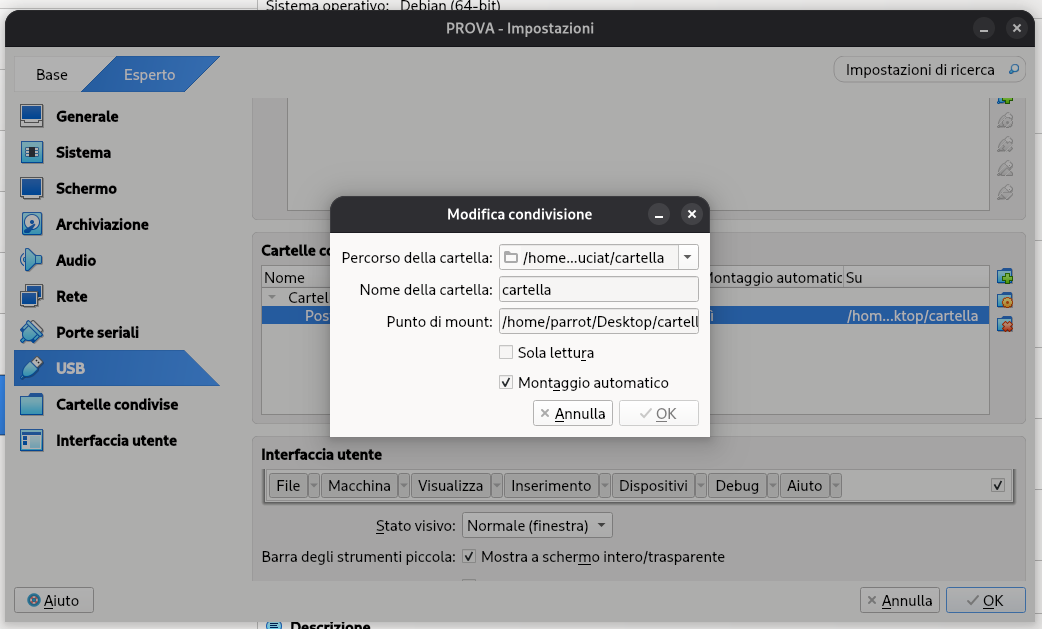
\includegraphics[width=0.85\textwidth]{shared_folder.png}
		\caption{In \textit{Impostazioni > Cartelle condivise}, aggiungere una nuova cartella: selezionare il percorso desiderato sull'host, impostare il punto di mount su \texttt{/home/parrot/Desktop/<nome\_cartella>} e spuntare \textbf{Montaggio automatico}.}
		\label{fig:shared_folder}
	\end{figure}
	
	% ─────────────────────────────────────────────
	\section{Creazione dello snapshot iniziale}
	
	Prima di avviare la macchina per la prima volta, è buona pratica creare uno snapshot \textit{pulito} della VM appena configurata.
	
	\begin{figure}[H]
		\centering
		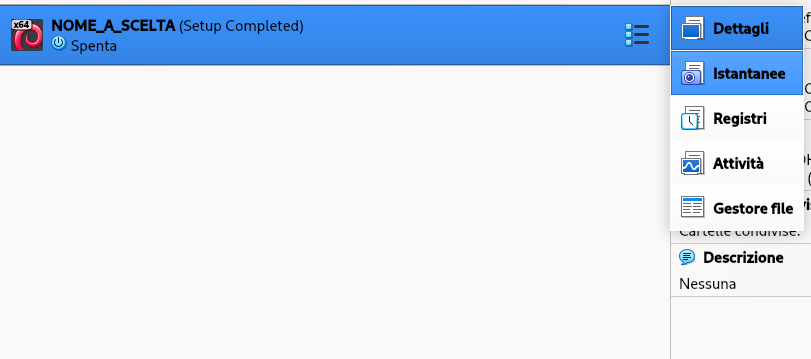
\includegraphics[width=0.85\textwidth]{select_snapshot_view.png}
		\caption{Dalla schermata principale di VirtualBox, cliccare sui tre puntini a destra del nome della VM e selezionare \textbf{Istantanee} (o \textit{Snapshots}) per aprire la vista dedicata.}
		\label{fig:select_snapshot}
	\end{figure}
	
	\begin{figure}[H]
		\centering
		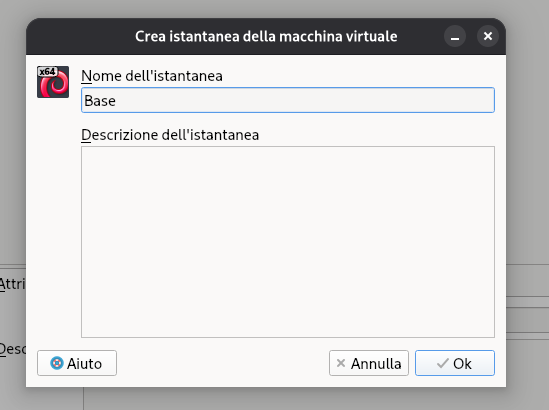
\includegraphics[width=0.85\textwidth]{base_snapshot.png}
		\caption{Cliccare su \textbf{Crea} e assegnare un nome allo snapshot (es. \textit{Base}), quindi confermare con \textbf{OK}.}
		\label{fig:base_snapshot}
	\end{figure}
	
	% ─────────────────────────────────────────────
	\section{Prima accensione e setup}
	
	Avviare la macchina virtuale ed eseguire le operazioni di configurazione iniziale.
	
	\begin{figure}[H]
		\centering
		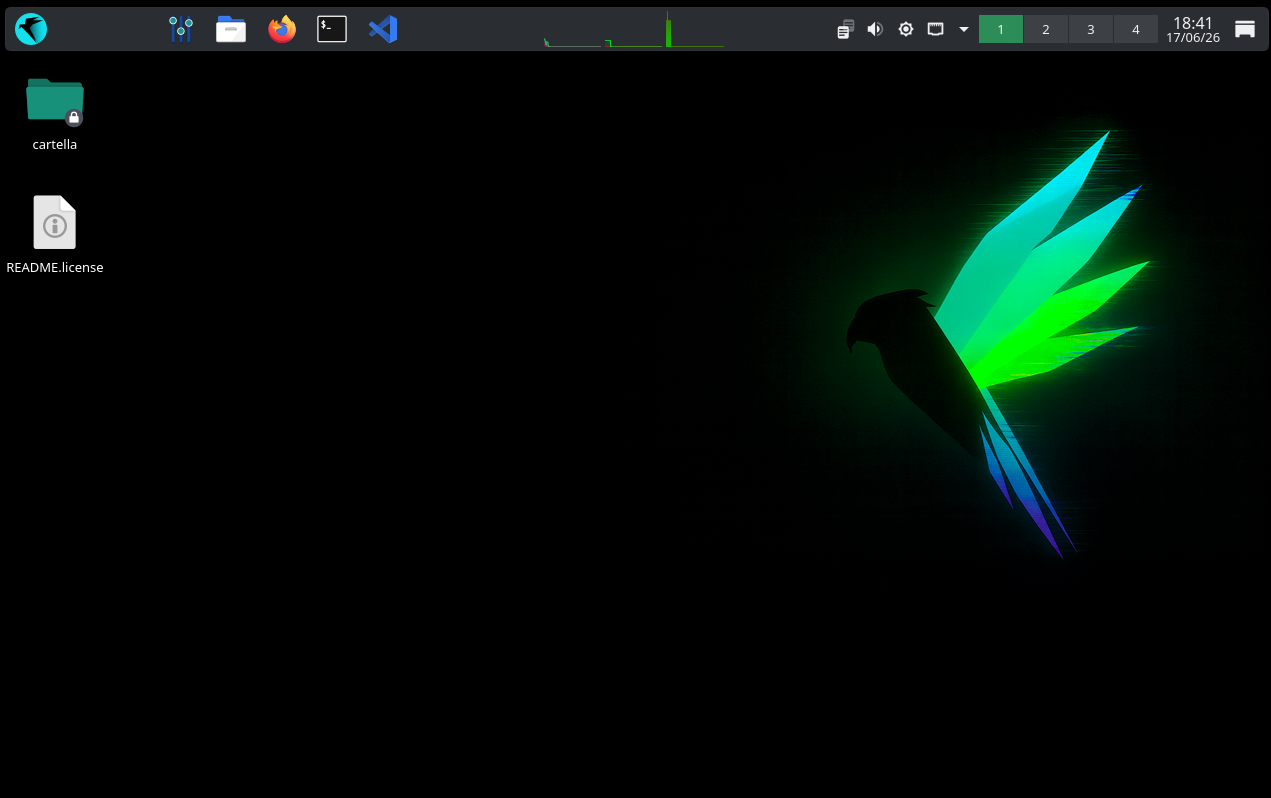
\includegraphics[width=0.85\textwidth]{locked_folder.png}
		\caption{Al primo avvio, la cartella condivisa sul desktop risulta bloccata (icona con lucchetto): è necessario aggiungere l'utente al gruppo corretto per potervi accedere.}
		\label{fig:locked_folder}
	\end{figure}
	
	\begin{figure}[H]
		\centering
		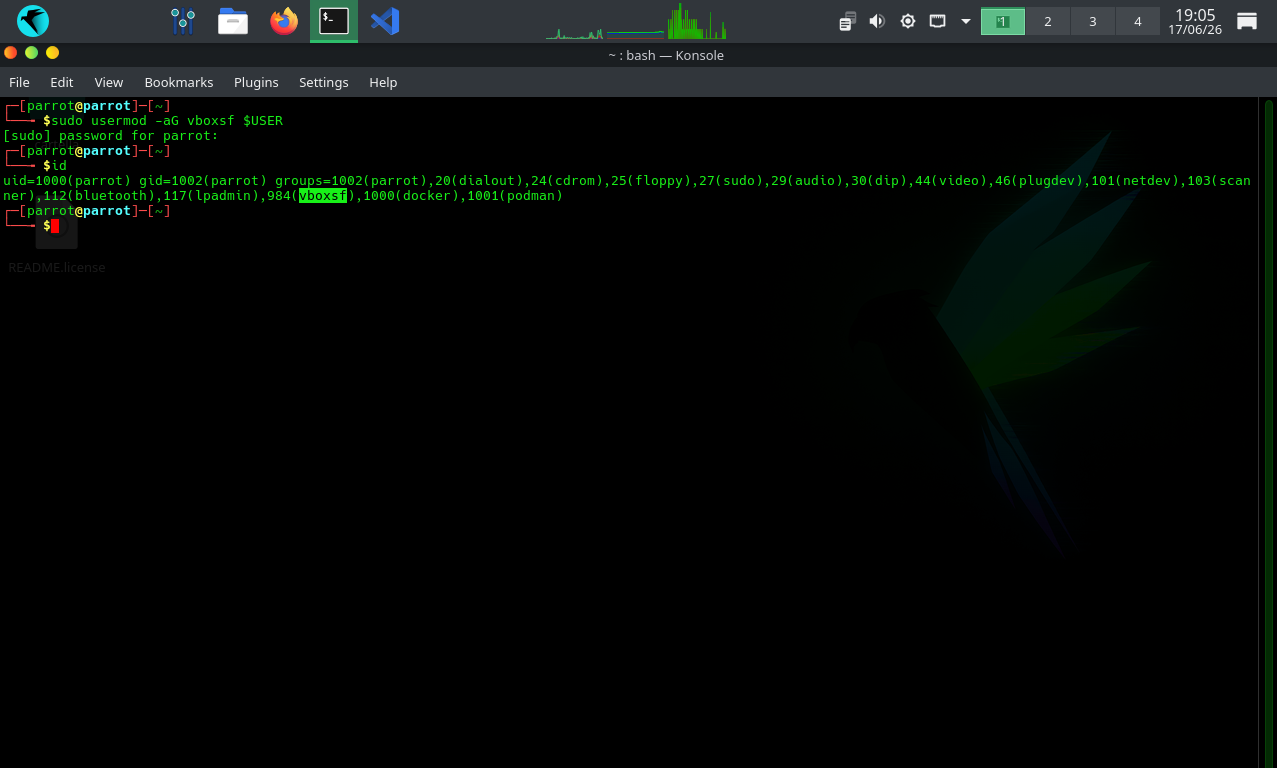
\includegraphics[width=0.85\textwidth]{add_vboxsf_group.png}
		\caption{Da terminale, eseguire il comando per aggiungere l'utente \texttt{parrot} al gruppo \texttt{vboxsf}, necessario per accedere alla cartella condivisa creata tramite VirtualBox.}
		\label{fig:add_group}
	\end{figure}
	
	\begin{figure}[H]
		\centering
		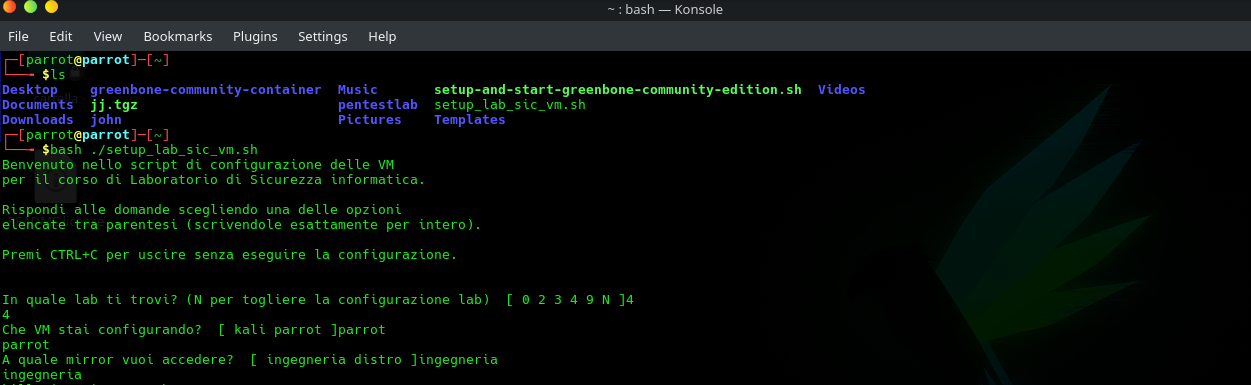
\includegraphics[width=0.85\textwidth]{script_setup.png}
		\caption{Eseguire lo script di setup fornito dai docenti. Lo script configura automaticamente l'ambiente; non è necessario alcun intervento manuale aggiuntivo.}
		\label{fig:script_setup}
	\end{figure}
	
	% ─────────────────────────────────────────────
	\section{Spegnimento e snapshot finale}
	
	Completato il setup, spegnere la macchina \textbf{senza salvare lo stato}, quindi creare uno snapshot definitivo.
	
	\begin{figure}[H]
		\centering
		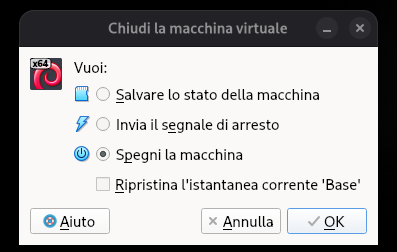
\includegraphics[width=0.85\textwidth]{turn_off.png}
		\caption{Alla chiusura della VM, selezionare \textbf{Spegni la macchina} (non \textit{Salva lo stato della macchina}) per eseguire uno spegnimento completo.}
		\label{fig:turn_off}
	\end{figure}
	
	Dopo lo spegnimento, creare un nuovo snapshot denominato \textbf{Setup completo} seguendo la stessa procedura descritta nella Sezione~\ref{fig:select_snapshot}.
	Al riavvio, la macchina sarà completamente operativa e la cartella condivisa risulterà accessibile e sbloccata.
	
	\begin{figure}[H]
		\centering
		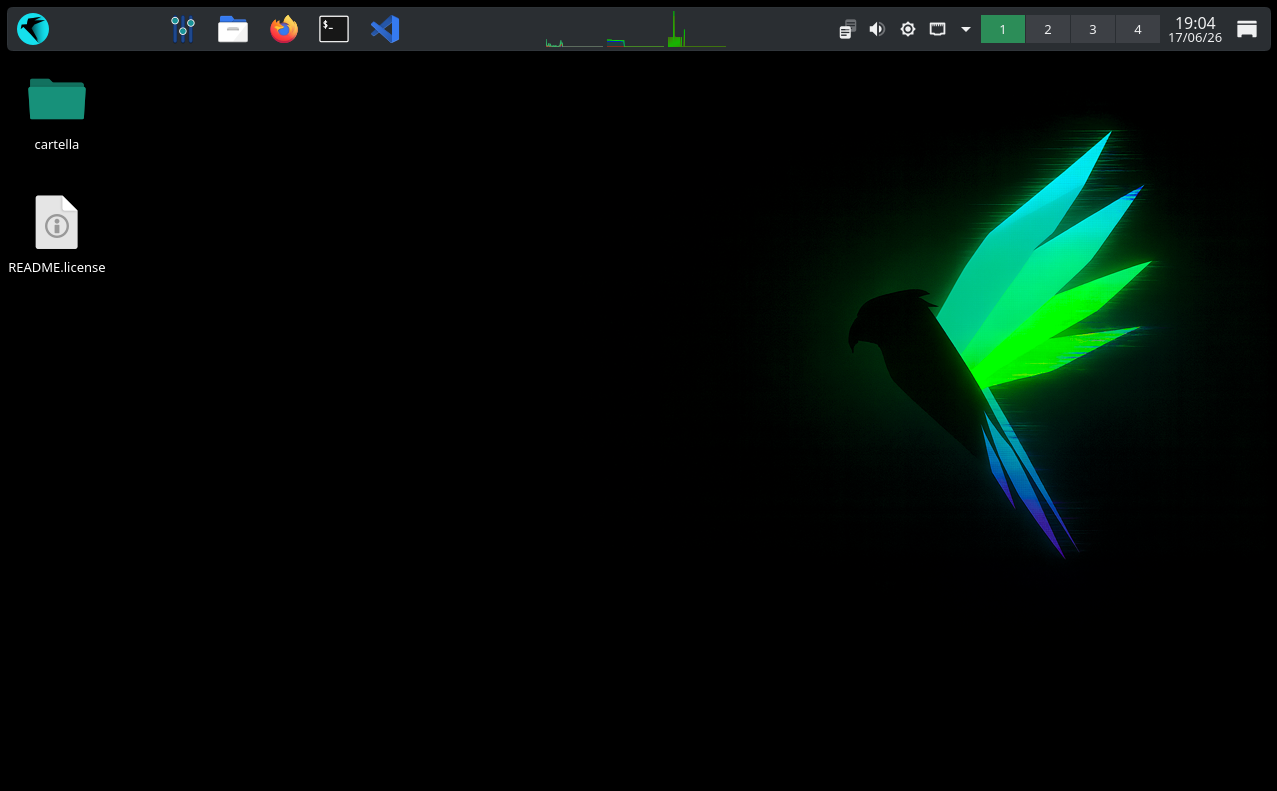
\includegraphics[width=0.85\textwidth]{unlocked_folder.png}
		\caption{Dopo il riavvio, la cartella condivisa sul desktop è ora accessibile (icona senza lucchetto). Lo snapshot \textit{Setup completo} permette di ripristinare questo stato in qualsiasi momento.}
		\label{fig:unlocked_folder}
	\end{figure}
	
\end{document}